% Physics experiment report
% 9/Dec/2016

\documentclass[a4paper,12pt,notitlepage]{article}

\usepackage{CJKutf8}
\usepackage{amsmath}
\usepackage{indentfirst}
\usepackage{float}
\usepackage{graphicx}
\usepackage{longtable}

\setlength{\parindent}{2em} 

\begin{CJK*}{UTF8}{gbsn}
\begin{document}

\title{RLC电路谐振实验报告}
\author{秦光辉\ 9组3号}
\maketitle

\section{实验数据处理}

	实验中保持以下参量不变:
	
\begin{align*}
	C &= 0.05 \mu C \\
	L &= 0.1 H \\
	R_L &= 18.016\Omega \\
	R &= (100.00 \pm 0.01) \Omega	
\end{align*}

	并联谐振实验中, 还保证
	
\begin{align*}
	R' = 5000.0 \Omega
\end{align*}

\subsection{串联谐振电路的第一种Q值与第二种Q值}

	当示波器上的利萨如图形成为直线时, 可以计算得到第一种Q值.
	
\begin{align*}
	f_0 &= 2.2482 kHz \\
	U_{tot} &= 0.6948 V \\
	U_R &= 0.5308 V \\
	R_{eff} &= R \times \frac{U_{tot}}{U_R} = 130.89 \Omega \\
	Q_1 &= \frac{1}{\omega CR_{eff}} = 10.81
\end{align*}

	同时可以估算其不确定度
	
\begin{align*}
	e_{U_{tot}} &= U_tot \times 0.2\% + 0.001V = 2.4 \times 10^{-3} \\
	e_{U_{R}} &= U_R \times 0.2\% + 0.001V = 2.1 \times 10^{-3} \\
	e_f &= 0.0005kHz \\
	e_C &= 0.65\% \times C = 0.000325 \mu C \\
	\sigma_{Q_1} &= \sqrt{\frac{1}{3}[(\frac{e_{U_{tot}}}{U_{tot}})^2 + (\frac{e_{U_R}}{U_R})^2 + (\frac{e_f}{f_0})^2 + (\frac{e_R}{R})^2 + (\frac{e_C}{C})^2]}\times Q_1 \\
	&= 0.0521 \\
	Q_1 \pm \sigma_{Q_1} &= 10.81 \pm 0.06
\end{align*}

	计算第二种品质因数, 有
	
\begin{align*}
	U_C &= 7.425V \\
	Q_2 &= \frac{U_C}{U_{tot}} = 10.69 \\
\end{align*}

	计算其不确定度, 有

\begin{align*}
	e_{U_C} &= U_C \times 0.2\% + 0.001V = 0.0159V \\
	\sigma_{Q_2} &= \sqrt{\frac{1}{3}[(\frac{e_{U_C}}{U_C})^2 + (\frac{e_{U_{tot}}}{U_{tot}})^2]}\times Q_2 \\
	&= 0.025 \\
	Q_2 \pm \sigma_{Q_2} &= 10.69 \pm 0.03
\end{align*}

\subsection{LRC串联谐振电路的相频曲线}

	实验数据见表一, 实验图线见图一. \\

\begin{center}

	\begin{longtable}{|c|c|c|c|c|c|c|c|}
	\caption{LRC串联谐振电路的相频数据} \\
	\hline
	f/kHz & 1.7600 & 1.9660 & 2.0720 & 2.1480 & 2.1900 & 2.2220 & 2.2482 \\
	\hline
	$\Delta$t/$mu$s & -124.5 & -101.5 & -82.0 & -59.5 & -38.0 & -19.0 & 0.0 \\
	\hline
	$\Delta \phi$ & -78.88 & -71.84 & -61.17 & -46.01 & -29.96 & -15.20 & 0.0 \\
	\hline
	\hline
	f/kHz & 2.2760 & 2.3090 & 2.3540 & 2.4340 & 2.5870 & 2.8900 &  \\
	\hline
	$\Delta$t/$mu$s & 19.5 & 35.5 & 55.0 & 70.0 & 77.5 & 78.5 &  \\
	\hline
	$\Delta \phi$ & 15.98 & 29.51 & 46.61 & 61.34 & 72.18 & 81.67 & \\
	\hline
	
	\end{longtable}

\end{center}

\begin{figure}[H]
\centering
	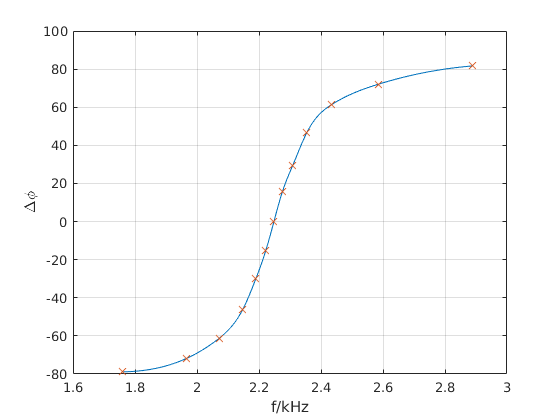
\includegraphics[scale=0.7]{exp14_1.png}
	\caption{LRC串联谐振电路的相频曲线}
\end{figure}

\subsection{LRC串联谐振电路的幅频曲线}

	实验数据见表二, 实验图线见图二. 实验中维持总电压为1.0000V左右. \\

\begin{center}

	\begin{longtable}{|c|c|c|c|c|c|c|c|}
	\caption{LRC串联谐振电路的幅频数据} \\
	\hline
	f/kHz & 1.7600 & 1.8600 & 1.9660 & 2.0150 & 2.0720 & 2.1120 & 2.1480 \\
	\hline
	$U_{tot}$/V & 0.9999 & 1.0000 & 1.0000 & 1.0001 & 1.0000 & 1.0000 & 1.0000 \\
	\hline
	$U_R$/V & 0.14055 & 0.18022 & 0.24859 & 0.29702 & 0.3770 & 0.4549 & 0.5450 \\
	\hline
	i/A & 0.014055 & 0.018022 & 0.024859 & 0.029702 & 0.03770 & 0.04549 & 0.05450 \\
	\hline
	\hline
	f/kHz & 2.1700 & 2.1900 & 2.2070 & 2.2220 & 2.2350 & 2.2482 & 2.2620 \\
	\hline
	$U_{tot}$/V & 1.0000 & 1.0000 & 1.0001 & 1.0000 & 1.0000 & 1.0000 & 0.9999 \\
	\hline
	$U_R$/V & 0.6073 & 0.6656 & 0.7102 & 0.7416 & 0.7585 & 0.7645 & 0.7575 \\
	\hline
	i/A & 0.06073 & 0.06656 & 0.07102 & 0.07416 & 0.07585 & 0.07645 & 0.07575 \\
	\hline
	\hline
	f/kHz & 2.2760 & 2.2925 & 2.3090 & 2.3315 & 2.3540 & 2.3490 & 2.4340 \\
	\hline
	$U_{tot}$/V & 1.0000 & 0.9999 & 0.9999 & 0.9999 & 0.9999 & 1.0001 & 1.0001 \\
	\hline
	$U_R$/V & 0.7381 & 0.7035 & 0.6610 & 0.5997 & 0.5410 & 0.5535 & 0.3839 \\
	\hline
	i/A & 0.07381 & 0.07035 & 0.06610 & 0.05997 & 0.05410 & 0.05535 & 0.03839 \\
	\hline
	\hline
	f/kHz & 2.5105 & 2.5870 & 2.7385 & 2.8900 &   & &   \\
	\hline
	$U_{tot}$/V & 1.0001 & 1.0001 & 1.0001 & 1.0001  &  &   & \\
	\hline
	$U_R$/V & 0.2947 & 0.23803 & 0.17300 & 0.13672 &  &   &  \\
	\hline
	i/A & 0.02947 & 0.023803 & 0.017300 & 0.013672 &  &    & \\
	\hline
	\end{longtable}

\end{center}

	从图中可以计算得到$Q_3$的值.

\begin{align*}
	f_1 &= 2.1470kHz \\
	f_2 &= 2.3550kHz \\
	\Delta f &= 0.2080 kHz \\
	f_0 &= 2.2482kHz \\
	Q_3 &= \frac{f_0}{\Delta f} = 10.81
\end{align*}

\begin{figure}[H]
\centering
	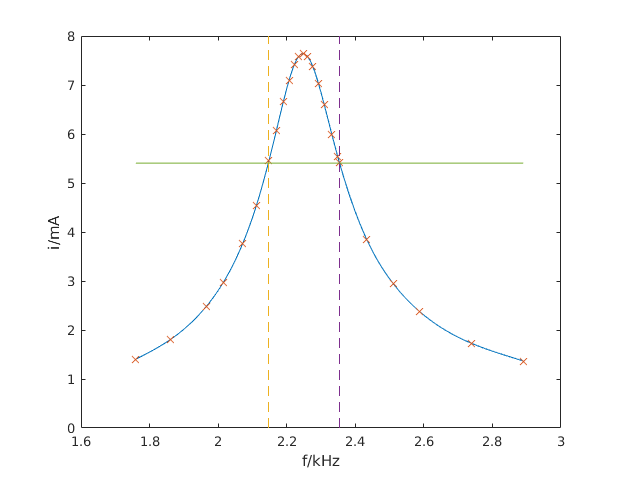
\includegraphics[scale=0.7]{exp14_2.png}
	\caption{LRC串联谐振电路的幅频曲线}
\end{figure}

\subsection{LRC并联谐振电路的相频曲线}

	并联谐振下, 谐振的频率为
	
\begin{align*}
	f_0 = 2.2451kHz
\end{align*}

\begin{center}

	实验数据见表三, 实验图线见图三. \\

	\begin{longtable}{|c|c|c|c|c|c|c|c|}
	\caption{LRC并联谐振电路的相频数据} \\
	\hline
	f/kHz & 1.7000 & 1.8000 & 1.9000 & 2.0000 & 2.0500 & 2.1000 & 2.1500 \\
	\hline
	$\Delta$/$\mu$s & 122 & 112 & 102 & 89 & 79 & 67.5 & 50.0 \\
	\hline
	$\Delta\phi$ & 74.66 & 72.58 & 67.77 & 64.08 & 58.30 & 51.03 & 38.70 \\
	\hline
	\hline
	f/kHz & 2.2000 & 2.2451 & 2.3000 & 2.3500 & 2.4000 & 2.5000 & 2.6000 \\
	\hline
	$\Delta$/$\mu$s & 22.5 & 0.0 & 38.5 & 60.0 & 68.5 & 78.0 & 80.5 \\
	\hline
	$\Delta\phi$ & 17.82 & 0.00 & -31.88 & -50.76 & -59.18 & -70.20 & -75.35 \\
	\hline
	\hline
	f/kHz & 2.7000 & 2.8000 & & & & &  \\
	\hline
	$\Delta$/$\mu$s & 83.5 & 81.0 & & & &  & \\
	\hline
	$\Delta\phi$ & -81.16 & -81.65 & & & & & \\
	\hline
	\end{longtable}

\end{center}

\begin{figure}[H]
\centering
	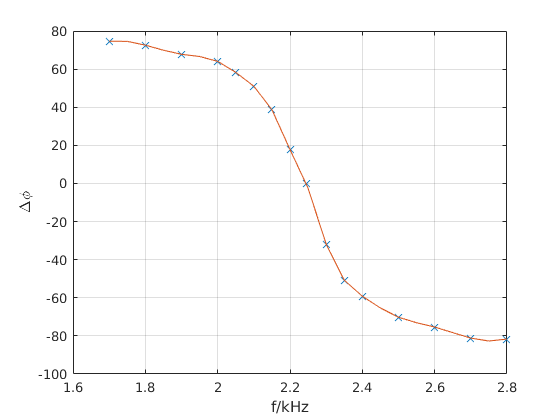
\includegraphics[scale=0.7]{exp14_3.png}
	\caption{LRC并联谐振电路的相频曲线}
\end{figure}

\subsection{LRC并联谐振电路的幅频曲线}

	实验数据见表四, 实验图线见图四. 实验中维持电阻箱两端电压为0.7000V. \\

\begin{center}

	\begin{longtable}{|c|c|c|c|c|c|c|c|}
	\caption{LRC并联谐振电路的幅频数据} \\
	\hline
	f/kHz & 1.7000 & 1.8000 & 1.9000 & 2.0000 & 2.0500 & 2.1000 & 2.1500 \\
	\hline
	$U_{R'}$/V & 0.7000 & 0.7000 & 0.6999 & 0.7000 & 0.6999 & 0.7000 & 0.7000 \\
	\hline
	$U_{tot}$/V & 0.3512 & 0.4408 & 0.5707 & 0.8020 & 0.9731 & 1.2193 & 1.5892 \\
	\hline
	\hline
	f/kHz & 2.2000 & 2.2451 & 2.3000 & 2.3500 & 2.4000 & 2.5000 & 2.6000 \\
	\hline
	$U_{R'}$/V & 0.7001 & 0.7000 & 0.7000 & 0.6999 & 0.7000 & 0.7000 & 0.7000 \\
	\hline
	$U_{tot}$/V & 1.9614 & 2.1412 & 1.8956 & 1.5210 & 1.2165 & 0.8437 & 0.6405 \\
	\hline
	\hline
	f/kHz & 2.7000 & 2.8000 & & & & &  \\
	\hline
	$U_{R'}$/V & 0.6999 & 0.7001 & & & & & \\
	\hline
	$U_{tot}$/V & 0.5174 & 0.4351 & & & & & \\
	\hline
	\end{longtable}

\end{center}

\begin{figure}[H]
\centering
	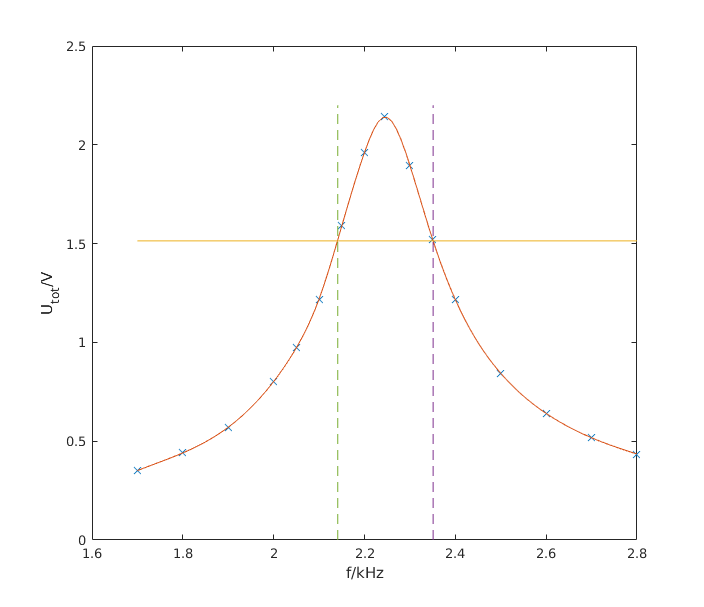
\includegraphics[scale=0.6]{exp14_4.png}
	\caption{LRC并联谐振电路的幅频曲线}
\end{figure}
	
	从图中可以计算得到$Q_3$的值.	
	
\begin{align*}
	f_1 &= 2.1410 kHz \\
	f_2 &= 2.3510 kHz \\
	\Delta f &= 0.2100 kHz \\
	f_0 &= 2.2451 kHz \\
	Q_3 &= \frac{f_0}{\Delta f} = 10.69
\end{align*}

\section{思考题}

\subsection{串联谐振中, 如果把电阻改成500$Omega$, 电路谐振特性会有什么变化?}

	由于$\omega_0 = \frac{1}{\sqrt{LC}}$, 故电阻的改变不会影响谐振频率. \\
	
	但是由于电阻的增大, 电路中阻抗也会增大, 电流会随之下降到五分之一. 考虑到电路还有其他阻值(如电感阻值), 最终电流应该略高于初始值的五分之一. \\
	
	由于$Q = \frac{1}{\omega_0 RC}$, 所以这个时候品质因数会下降到原来的五分之一左右. 电路的频率选择性会变差 \\
	
	对于相频曲线, 有
	
\begin{align*}
	tan\Delta\phi = \frac{\omega L - \frac{1}{\omega L}}{R}
\end{align*}

	随着电阻的增大, 上式变小, 所以相频曲线会变缓.
	
\subsection{思考题(2)}

\subsubsection{说明测量原理}

	调节电路, 使得电路达到谐振状态, 然后测量总电压和电容上的电压, 最后得到
	
\begin{align*}
	Q = \frac{U_C}{U_{tot}}
\end{align*}

\subsubsection{测量步骤}

\begin{enumerate}
	\item 调节信号源的频率, 使电容上的电压达到极大值, 这个时候电路达到谐振状态
	\item 读毫伏表, 得到总电压$U$和电容器上的电压$U_C$
\end{enumerate}

\subsubsection{若在测某样品时, C = 330 pF, $f_0$ = 600 kHz, U = 10 mV, $U_C$ = 1.00 V, 试求L, $R_r$, Q值}

\begin{align*}
	L &= \frac{1}{4\pi^2f_0^2C} = 0.2132mH \\
	R_r &= \frac{U}{i} = \frac{U}{2\pi f_0CU_C} = 8.0\Omega \\
	Q &= \frac{U_C}{U} = 1.0 \times 10^2
\end{align*}

\section{分析与讨论}

\subsection{实验中测得的各种曲线有什么特征? 如何理解? }

\subsubsection{串联电路的相频曲线}

	电流与电压的相位差在谐振的时候为0, 在频率为正无穷和负无穷的时候趋近于90度与-90度. \\
	
	在低频的时候, 电容的容抗是电路阻抗的主要组成部分, 此时电压相位会落后于电流相位. 在谐振的时候, 电容和电感的阻抗相互抵消, 电路呈现纯电阻性, 自然电流和电压没有相位差. 在高频的时候, 电感成为阻抗的主要组成部分, 电压相位落后于电流相位. 

\subsubsection{串联电路的幅频曲线}

	串联谐振曲线的电流大小可以用下式计算.
	
\begin{align*}
	|\tilde{i}| = |\frac{\tilde{u}}{-\frac{1}{i\omega C} + i\omega L + R}|
\end{align*}

	实验中保持总电压不变, 所以电流应该呈现单峰性, 在谐振的时候达到极值. 实际情况确实和理论计算完全相同. 在频率很小或者很大的时候, 电流趋近于0.

\subsubsection{并联电路的相频曲线}

	图线和串联谐振电路类似, 但是趋势恰好相反. \\

	低频情况下, 电容的容抗很大, 电感的感抗很小. 此时电压的相位超前于电流相位. 当频率逐渐增大, 达到谐振频率的时候, 相位差为0. 频率继续增大的时候, 相位差变成负值. \\
	
	以上现象可以如此定性理解: 在并联电路中, 当频率较低的时候, 电容的容抗很大. 不妨取一个极限, 电路是直流电路, 此时电容为短路, 电感和电阻组成的支路电阻较低, 所以电路应该呈现感性, 所以电压相位应该超前于电流.

\subsubsection{并联电路的幅频曲线}

	和串联电路的幅频曲线类似, 图线呈现单峰性. 在谐振的时候电压达到最大值. \\

	电路的电压可通过下式计算:
	
\begin{align*}
	|\tilde{u_{tot}}| = |\tilde{i}\frac{(R + i\omega L)(\frac{-i}{\omega C})}{R + i\omega L + \frac{-i}{\omega C}}|
\end{align*}

	实际测得的曲线和理论相符.
	
\subsection{分析三种方法得到的Q值}

	三个Q值的大小关系是
	
\begin{align*}
	Q_1 \approx Q_3 > Q_2
\end{align*}

	造成这种现象的原因可能是电表阻值并联入电路引起的. 电表的阻值为1M$\Omega$, 这个阻值还不够大. 在串联电路中, 电容的容抗约为
	
\begin{align*}
	\frac{1}{\omega C} = 1.4 k\Omega
\end{align*}

	此时电表的内阻就会对测量产生影响. 而电路总电阻仅为100$\Omega$量级, 所以总电压测量不会有偏差. 所以$Q_2$可能会偏小. \\
	
	测量$Q_1$的时候, 用电压的比值来间接获得电路的总电阻. 测量$Q_3$的时候, 用作图法来获得$\Delta f$. 这两种方法都有很大误差, 所以数据也不是非常可信.

\section{思考和感悟}

	实验从原理到操作都不算复杂, 但是我却出现了很多小问题. 实验中我接错了电路, 导致很大一部分数据都得重测. 我觉得我做实验的技能还有待提高. 欲速则不达, 我不应该做那么着急. 特别是电路实验, 这次虽然没有出现事故, 但是日后如果操作高压电路, 这样的错误不能犯.
	
\end{CJK*}
\end{document}
